\section{Label Distribution}
We started by analyzing the distribution of the labels in the dataset. The distribution of the labels is shown in Figure \ref{fig:label_dist}.
\begin{figure}[H]
    \vspace*{0.7cm}
    \centering
    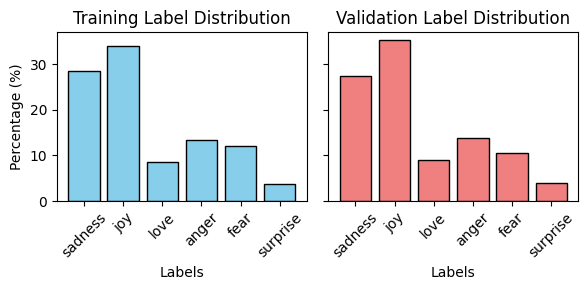
\includegraphics[width=0.22\textwidth]{figures/label_dist.png}
    \caption{Distribution of the labels in the dataset.}
    \label{fig:label_dist}
    \vspace*{0.7cm}
\end{figure}
As can be seen, the dataset is very unbalanced, with the majority of the tweets being labeled as joy or sadness. This could potentially lead to the model being biased towards these labels.